\documentclass[12pt,a4paper]{article}

\usepackage[a4paper,margin=2.5cm]{geometry}
\usepackage{fontspec}
\setmainfont{Times New Roman}
\usepackage{setspace}
\onehalfspacing
\usepackage{hyperref}
\usepackage{longtable}
\usepackage{booktabs}
\usepackage{enumitem}
\usepackage{graphicx}
\setlength{\emergencystretch}{3em}

\title{Premade Graph adatbázis projekt dokumentáció}
\author{Adatbázisrendszerek projekt}
\date{2026}

\begin{document}

\maketitle

\section{Bevezetés}

A Premade Graph egy adatbázisra épülő League of Legends játékos-hálózati elemző rendszer. A projekt célja meccselőzmények és játékosadatok gyűjtése, ismétlődő együttjátszások és ellenfélkapcsolatok gráffá alakítása, valamint olyan elemzési eredmények tárolása, mint a klaszterek, játékos-teljesítmény mutatók, útkeresési lekérdezések és aláírt gráf alapú kapcsolati eredmények.

A téma napjainkban azért fontos, mert az esport rendszerek nagy mennyiségű strukturált digitális nyomot hoznak létre. Egy MOBA játékban nemcsak az eredmény érdekes, hanem a játékosok szerepe, csapathoz tartozása, teljesítménye, ismétlődő kapcsolata és közösségi szerkezete is. A Premade Graph adatbázisa ezért nem egyszerű játékoslista, hanem elemzési célú relációs modell.

A rendszer fő célkitűzései:

\begin{itemize}
  \item játékosok, meccsek, csapatok és résztvevők normalizált tárolása;
  \item ismétlődő szövetséges és ellenfél kapcsolatok tárolása;
  \item gráfelemzési eredmények, klaszterek és útkeresések mentése;
  \item teljesítménymutatók kezelése, például \texttt{opscore} és \texttt{feedscore};
  \item nézetek, összetett lekérdezések, tárolt eljárások és triggerek biztosítása.
\end{itemize}

A beadandó adatbázis-változat PostgreSQL-re készült, mert a feladat tárolt eljárásokat, triggereket, rekurzív lekérdezéseket, JSON mezőket és összetettebb SQL elemzéseket is kér. A tényleges alkalmazás jelenleg SQLite-ot használ helyi perzisztenciára, de a dokumentált modell ugyanazokat a fogalmakat viszi át egy erősebb adatbázisrendszerbe.

\section{Szakirodalmi kutatás}

A League of Legends és MOBA elemzésekkel foglalkozó szakirodalom alátámasztja a választott adatbázismodellt. Mora-Cantallops és Sicilia szerint a MOBA játékok fontos kutatási területet jelentenek, mert egyszerre jelenik meg bennük verseny, együttműködés, játékosélmény és társas interakció [1]. Ez indokolja, hogy az adatbázis ne csak meccseredményeket, hanem játékoskapcsolatokat is tároljon.

Bahrololloomi és munkatársai League of Legends játékos-teljesítmény metrikákat vizsgálnak, és olyan adatgyűjtési megközelítést írnak le, amely kiválasztott játékosokból indul ki, majd a friss meccsek alapján további játékosokat von be [2]. Ez szorosan kapcsolódik a Premade Graph működéséhez, ahol a meccsgyűjtés új játékosokat fedez fel, majd teljesítményértékeket számol. A szerepkörfüggő elemzés miatt a szerep és az ösvény adatai nemcsak a játékosnál, hanem a meccsrésztvevő rekordban is szerepelnek.

Novak és munkatársai profi League of Legends meccsek teljesítményét modellezik szakértői mutatók alapján [3]. Ez azt mutatja, hogy az esport elemzéseknél fontos a strukturált változók és a domainismeret használata. Emiatt a javasolt adatbázis külön tárolja a nyers résztvevői adatokat, például kill, death és assist értékeket, valamint a származtatott mutatókat, például \texttt{opscore}, \texttt{feedscore} és volatilitás.

Ghawi, Müller és Pfeffer megmutatják, hogy az időbeli kommunikációs hálózatok javíthatják az online játékok csapatteljesítményének előrejelzését [4]. Ez indokolja az időbélyegzett meccsek, elemzési futások és teljesítmény-pillanatképek tárolását. Egy statikus játékostábla nem elegendő, mert a longitudinális elemzéshez tudni kell, mikor figyeltük meg az adatot és mikor számoltuk az eredményt.

Sánchez és González-Bailón a profi League of Legends csapathatékonyságát hálózati szerkezettel kötik össze [5]. Ez támogatja a \texttt{player\_relationships}, \texttt{clusters} és \texttt{cluster\_members} jellegű táblák használatát. Az adatbázisnak lehetővé kell tennie a belső klasztersűrűség, hídjátékosok és kapcsolat-erősségek vizsgálatát.

A játékosközpontú League of Legends hálózatkutatás szintén alátámasztja a gráfmutatók és ego-hálózati tulajdonságok tárolását [6]. A Premade Graph ezt az elvet alkalmazza, amikor a játékosokat csúcsokként, az ismétlődő ally/enemy bizonyítékokat pedig élekként kezeli. A friss, strukturált meccsösszegzéssel foglalkozó kutatás tovább erősíti azt az igényt, hogy a nyers JSON-szerű meccsadatok tömör, lekérdezhető szerkezetbe kerüljenek [7].

\section{Rendszerkövetelmények}

\subsection{Funkcionális követelmények}

\begin{enumerate}
  \item A rendszer tárolja a játékosok azonosítóját, nevét, régióját, szerepét és teljesítménypontszámait.
  \item A rendszer tárolja a meccsek sorát, patch verzióját, régióját, kezdési idejét, hosszát és győztes oldalát.
  \item A rendszer tárolja a csapatokat és a meccsrésztvevőket, hogy minden játékos egy adott meccs adott csapatához köthető legyen.
  \item A rendszer tárolja a játékosok közötti szövetséges és ellenfél kapcsolatokat súllyal és bizonyítékszámmal.
  \item A rendszer tárolja a közösségdetektálási és klaszterezési eredményeket.
  \item A rendszer tárolja az elemzési futások során számolt teljesítmény-pillanatképeket.
  \item A rendszer tárolja az útkeresési kéréseket és eredményeket.
  \item A rendszer biztosítson elemző nézeteket játékos-teljesítményhez és klaszterállapothoz.
  \item A rendszer tartalmazzon összetett lekérdezéseket riportoláshoz, szűréshez, rangsoroláshoz, JSON kezeléshez és aggregációhoz.
  \item A rendszer tartalmazzon tárolt eljárásokat, függvényeket és triggereket az ismételhető adatbázislogikához.
\end{enumerate}

\subsection{Nem funkcionális követelmények}

\begin{enumerate}
  \item A séma legyen normalizált, hogy ne duplikálja feleslegesen a játékos- és meccsadatokat.
  \item Az elemzési eredmények legyenek reprodukálhatók külön elemzési futás rekordokkal.
  \item A gyakori kapcsolásokhoz indexek tartozzanak.
  \item A séma őrizze meg a hivatkozási integritást elsődleges és idegen kulcsokkal.
  \item A származtatott értékek különüljenek el a nyers megfigyelésektől.
  \item Az adatbázis támogassa a JSON metaadatokat, de ne helyettesítse velük a relációs szerkezetet.
  \item A lekérdezések legyenek érthetők dokumentációs és bemutatási célra is.
\end{enumerate}

\section{Rendszerarchitektúra és részletes terv}

Az architektúra négy logikai rétegből áll. Az adatgyűjtési réteg játékos- és meccsmegfigyeléseket szerez be. A perzisztencia réteg PostgreSQL táblákban tárolja a normalizált adatokat. Az elemzési réteg gráfkapcsolatokat, klasztereket, teljesítményösszegzéseket és útkeresési eredményeket számol. A megjelenítési réteg ASP.NET Core adatbázis-böngészőként mutatja be a generált projektadatbázist.

\subsection{Egyed-kapcsolat modell}

A központi egyed a \texttt{players}. A meccsek a \texttt{matches}, \texttt{teams} és résztvevői táblákon keresztül jelennek meg. Ez megakadályozza, hogy ugyanazok a meccsszintű adatok minden játékosnál ismétlődjenek. A játékos-játékos gráfszerkezetet a kapcsolat tábla tárolja. A klasztereredmények a \texttt{clusters} és klasztertagsági táblában találhatók. Az elemzési történet elemzési futásokból, teljesítmény-pillanatképekből és útlekérdezésekből áll.

\subsection{Relációs táblák}

\begin{longtable}{p{4cm}p{10cm}}
\toprule
Tábla & Cél \\
\midrule
\texttt{players} & Játékosazonosság és aktuális összegzett pontszámok. \\
\texttt{matches} & Meccsszintű adatok, például queue, patch, időtartam és győztes. \\
\texttt{teams} & Egy meccs két csapata oldallal és objektíva adatokkal. \\
\texttt{match participants} & Egy játékos statisztikái egy meccsen és csapatban. \\
\texttt{player relationships} & Előjeles ally/enemy gráfélek a meccselőzményből. \\
\texttt{clusters} & Közösségdetektálási vagy útkeresési klasztereredmények. \\
\texttt{cluster members} & Több-a-több kapcsolat játékosok és klaszterek között. \\
\texttt{performance snapshots} & Időbélyegzett származtatott teljesítménymutatók. \\
\texttt{analysis runs} & Lefuttatott elemzési munkák metaadatai. \\
\texttt{path queries} & Elmentett útkeresési kérések és eredmények. \\
\bottomrule
\end{longtable}

A mappában található PlantUML, Mermaid és draw.io diagramok tartalmazzák az ER és relációs nézeteket.

\begin{figure}[htbp]
\centering
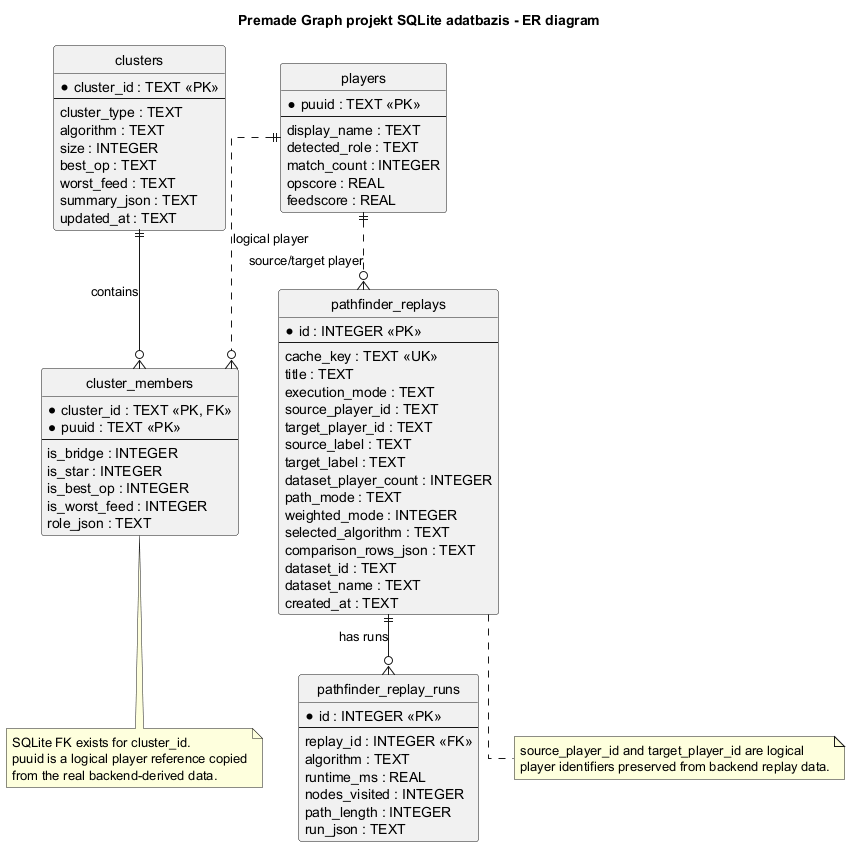
\includegraphics[width=\textwidth]{er_diagram.png}
\caption{A Premade Graph adatbázis fő ER kapcsolatai.}
\label{fig:er-diagram}
\end{figure}

\begin{figure}[htbp]
\centering
\small
\begin{tabular}{c}
\fbox{\begin{minipage}{0.62\textwidth}\centering \textbf{Backend adatbázisok}\\players.db, pathfinder\_replays.db, playersrefined.db\end{minipage}}\\[0.22cm]
$\Downarrow$\\[0.22cm]
\fbox{\begin{minipage}{0.62\textwidth}\centering \textbf{Automatikus import indításkor}\\kézi mód: dotnet run -- import\end{minipage}}\\[0.22cm]
$\Downarrow$\\[0.22cm]
\fbox{\begin{minipage}{0.62\textwidth}\centering \textbf{Datasetenkénti projekt SQLite adatbázis}\\Data/premadegraph\_project\_\{dataset\}.db\end{minipage}}\\[0.22cm]
$\Downarrow$\\[0.22cm]
\fbox{\begin{minipage}{0.62\textwidth}\centering \textbf{ASP.NET Core felület}\\adatbázis böngésző\end{minipage}}
\end{tabular}
\caption{Az egyszerű felület adatáramlása a valós backend adatbázisoktól a böngészhető projektadatbázisig.}
\label{fig:interface-dataflow}
\end{figure}

\section{Egyszerű felhasználói felület}

A beadandóhoz készült ASP.NET Core felület a \texttt{simple-interface} mappában található. A felület nem kézzel beírt adatokat jelenít meg, hanem generált SQLite projektadatbázist olvas. A datasetek a backend \texttt{data/datasets.json} regiszteréből érkeznek, például \texttt{default}, \texttt{flexset} vagy \texttt{soloq}. A böngészőben egyszerre egy dataset aktív, és minden dataset külön \texttt{Data/premadegraph\_project\_\{dataset\}.db} fájlba importálódik, ezért az adatforrások nem keverednek. Normál indításkor az alkalmazás automatikusan lefuttatja az importot az aktuális datasetre, a \texttt{dotnet run -- import flexset} jellegű parancs pedig kézi, csak importáló módként is elérhető. A kezdőoldal maga az adatbázis-böngésző: szerveroldali lapozással egyszerre csak az aktuális tábla aktuális oldalát tölti be. Támogatja a datasetválasztást, a globális keresést, az oszloponkénti szűrést, a rendezést, a tábla szerinti váltást és az oszlopmagyarázó súgókat. A nagyméretű JSON mezők, például az útkeresési futások teljes \texttt{run\_json} tartalma, nem kerülnek automatikusan a táblanézetbe; a böngésző rövid előnézetet mutat, a teljes mező külön oldalon nyitható meg.

\section{Eredmények}

Az adatbázisterv teljesíti a feladat fő elvárásait:

\begin{itemize}
  \item a \texttt{schema.sql} 10 táblát definiál;
  \item minden táblának legalább 5 attribútuma van;
  \item a \texttt{sample\_data.sql} legalább 10 sort tölt minden táblába;
  \item a \texttt{views\_queries.sql} két fontos nézetet tartalmaz;
  \item 20 különböző, nem csak névcserén alapuló lekérdezés készült;
  \item a \texttt{procedures\_triggers.sql} tárolt eljárásokat, rekurzív függvényt és triggereket tartalmaz;
  \item szerepel JSON lekérdezés, join, egymásba ágyazott select, aggregáció, \texttt{HAVING}, rekurzív CTE és \texttt{EXCEPT}.
\end{itemize}

A terv illeszkedik a jelenlegi Premade Graph projekthez is. A játékosok, klaszterek, gráfkapcsolatok és útkeresési eredmények elsőrangú adatbázis-elemként jelennek meg, így a rendszer alkalmas alkalmazásdemóra és szakdolgozati jellegű elemzésre is.

\section{Összegzés}

Ez a dokumentáció egy teljes relációs adatbázisprojektet mutat be a Premade Graph rendszerhez. A választott téma releváns, mert az esport meccsadatok alkalmasak egyéni teljesítmény, csapatviselkedés, gráfszerkezet és időbeli játékosstabilitás vizsgálatára. A szakirodalmi áttekintés alapján a League of Legends elemzése már létező kutatási irány, de értékes egy olyan rendszer, amely teljesítmény-, hálózati és időbeli adatokat egy adatbázismodellben kapcsol össze.

A PostgreSQL séma normalizált és elemzésorientált. Támogatja a nyers meccsrekordokat, a származtatott teljesítménymutatókat, az előjeles kapcsolatokat, a klasztereket és az útkeresési előzményeket. A tárolt eljárások és triggerek megmutatják, hogyan tartható konzisztensen az adatbázis oldali logika. A beadandó felülete a valós backend-adatokból generált SQLite adatbázist böngészi, ezért az elkészült dokumentáció, SQL csomag és ASP.NET Core alkalmazás egységesen bemutatható projektállapotot ad.

\section{Hivatkozások}

\begin{enumerate}
  \item Mora-Cantallops, M., \& Sicilia, M.-A. (2018). MOBA games: A literature review. \textit{Entertainment Computing}, 26, 128--138. \url{https://doi.org/10.1016/j.entcom.2018.02.005}
  \item Bahrololloomi, F., Klonowski, F., Sauer, S., Horst, R., \& Dörner, R. (2023). E-Sports player performance metrics for predicting the outcome of League of Legends matches considering player roles. \textit{SN Computer Science}, 4, 238. \url{https://doi.org/10.1007/s42979-022-01660-6}
  \item Novak, A. R., Bennett, K. J. M., Pluss, M. A., \& Fransen, J. (2020). Performance analysis in esports: Modelling performance at the 2018 League of Legends World Championship. \textit{International Journal of Sports Science and Coaching}, 15(5--6), 809--817. \url{https://doi.org/10.1177/1747954120932853}
  \item Ghawi, R., Müller, S., \& Pfeffer, J. (2021). Improving team performance prediction in MMOGs with temporal communication networks. \textit{Social Network Analysis and Mining}, 11, 65. \url{https://doi.org/10.1007/s13278-021-00775-7}
  \item Sánchez, P., \& González-Bailón, S. (2019). Team efficiency and network structure: The case of professional League of Legends. \textit{Social Networks}, 58, 105--115. \url{https://doi.org/10.1016/j.socnet.2019.03.004}
  \item Sánchez, P. (2019). Player-centric networks in League of Legends. \textit{Social Networks}. \url{https://doi.org/10.1016/j.socnet.2018.12.001}
  \item Kim, J., Lee, W., \& Park, J. (2025). Structured summarization of League of Legends match data optimized for large language model input. \textit{Applied Sciences}, 15(13), 7190. \url{https://doi.org/10.3390/app15137190}
\end{enumerate}

\end{document}
